\clearpage
\section{Statistical Analysis}
\paragraph{Mode selection}
With large datasets, previous "event display" method will no longer be efficient and accurate. Thus data analysis tools are necessary. Here \verb|root| is used and three macros to apply cuts are already implemented. As before we have four sets of Monte Carlo simulated data in order to find the optimal cuts, then there are a couple of real data samples.

First of all, there are a couple of general cuts. The collider energy of LEP is $\sim\SI{200}{\giga\eV}$. Thus the scalar sum of momenta should be maximally around this value. Events with even larger momenta are caused by various unphysical processes. Secondly, the data here is written such as when there are multiple outgoing positive particles, $\verb|cos_thet|=1000$. For $ee$ and $\mu\mu$ process, it should not be possible, since no hadronisation can occur and initial/final state radiation for these two only involve photons. So for these two event selections, cut $\verb|cos_thet| <= 1.0$ is applied, see figure~\ref{fig:cos_thet_cut}. After the cut(s), there are $56613$ $ee$ events, $89646$ $\mu\mu$ events, $79099$ $\tau\tau$ events, and $98100$ $qq$ events.
\begin{figure}[ht]
	\centering
	\includegraphics[width=0.8\linewidth]{cos_thet_before.pdf}
	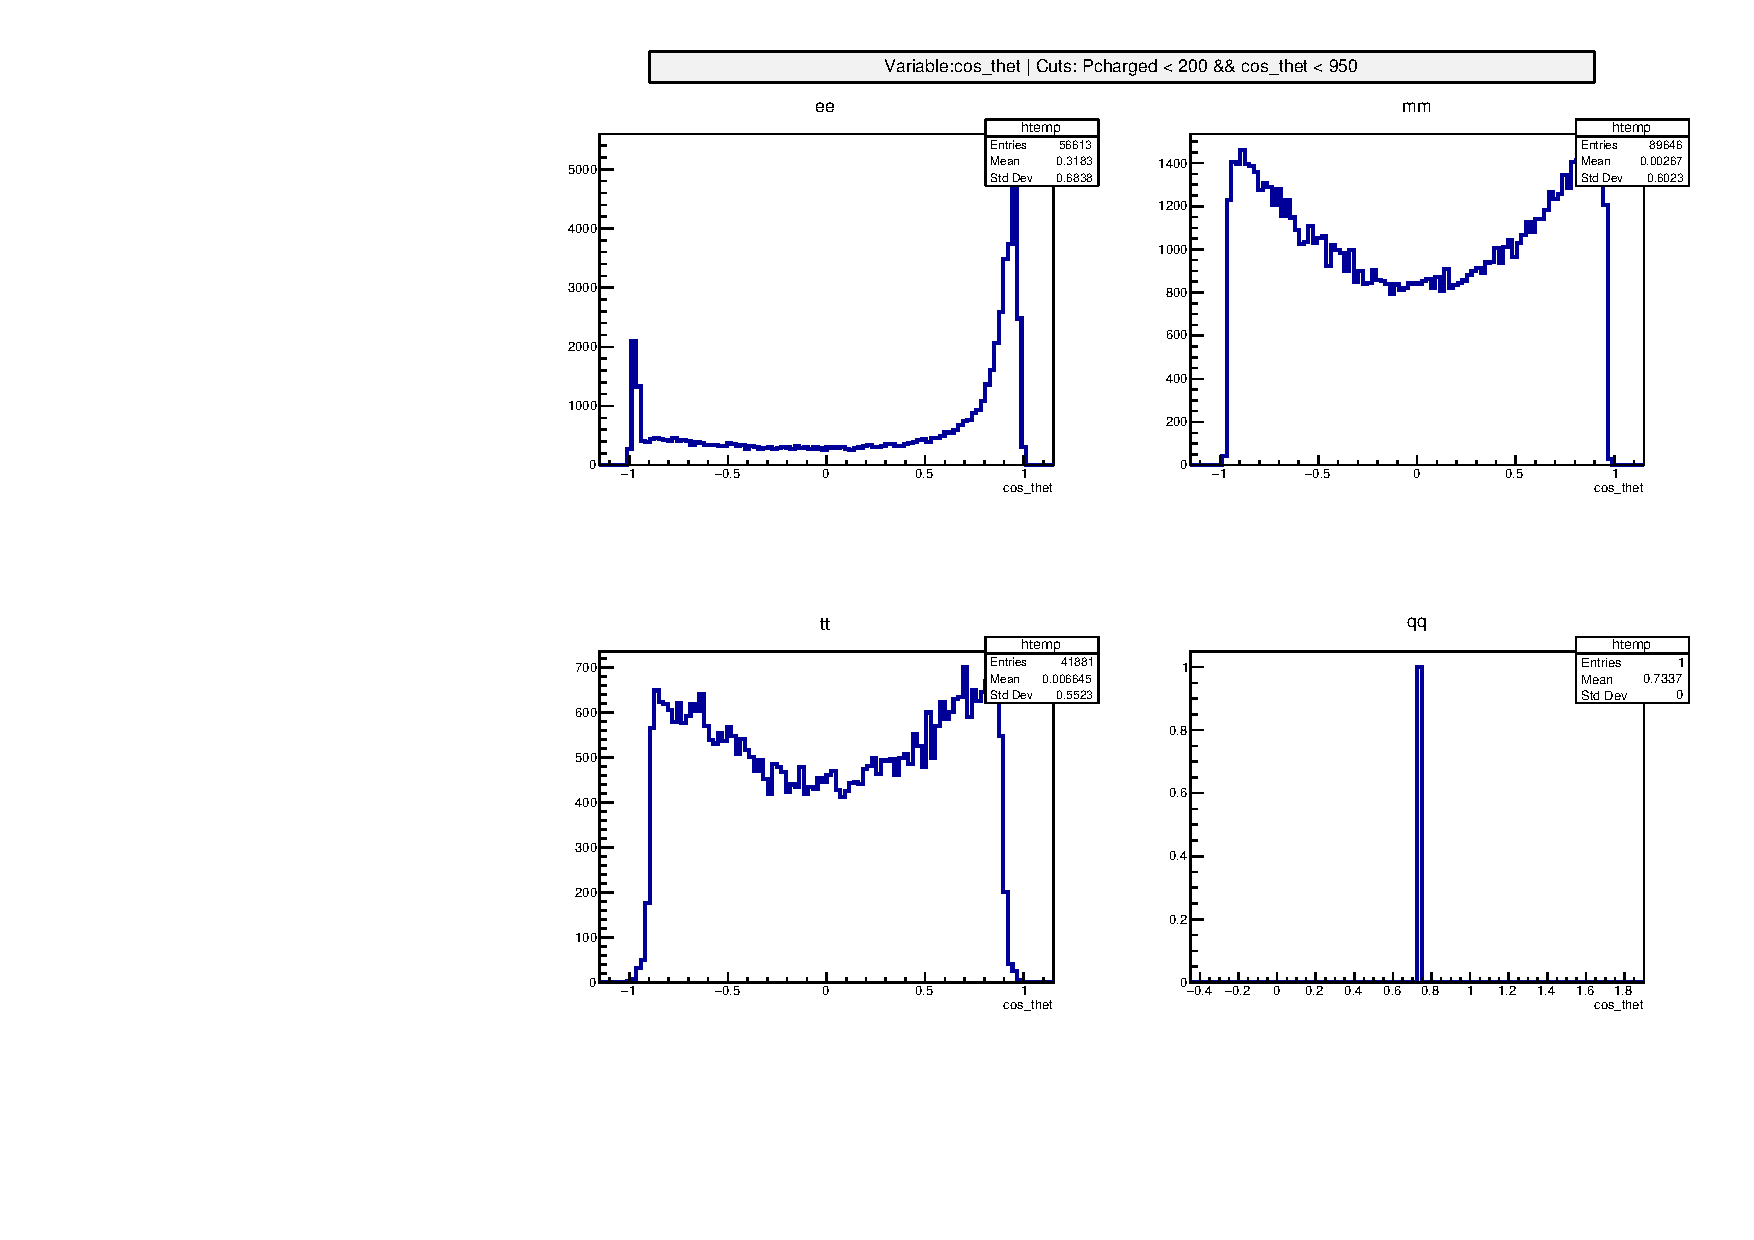
\includegraphics[width=0.8\linewidth]{cos_thet_after.pdf}
	\cprotect\caption{Distribution of \verb|cos_thet| before and after \verb|cos_thet| cut.}%
	\label{fig:cos_thet_cut}
\end{figure}

\clearpage
In event display part, we had success using cut $\verb|Ncharged| > 7$ for $qq$ processes. We conclude that this is no longer sufficient, since there are quite many $\tau\tau$ contamination, see figure~\ref{fig:qq_Ncharged_cuts}. While roughly $5\%$ percent of $qq$ events are lost, $\tau\tau$ events are barely present and $ee$, $\mu\mu$ are completely cut. So the $5\%$ percent are considered as acceptable "casualties". After the cut for $qq$, no $ee$ or $\mu\mu$ are left, $78$ $\tau\tau$ survives and $92688$ $qq$ events remain.
\begin{figure}[ht]
	\centering
	\includegraphics[width=0.8\linewidth]{N_charged_before2.pdf}
	\includegraphics[width=0.8\linewidth]{N_charged_after.pdf}
	\cprotect\caption{Number of charged tracks (\verb|Ncharge|) before and after the refined cut for $qq$ events.}%
	\label{fig:qq_Ncharged_cuts}
\end{figure}

Follow the same receipt as in event display part, we try to separate $ee$ events from other leptonic channels. Cut in number of charged track remains the same: $\verb|Ncharged| < 4 $ or ($\leq 3$). Same as before \verb|E_ecal| of $ee$ events have peak at around \SI{80}{\giga\eV}. \verb|E_ecal| cut is changed to $\verb|E_ecal| > 60$, since there is virtually no events even at $\verb|E_ecal| = 60$, see figure~\ref{fig:ee_cuts}. \verb|E_hcal| cut is similar to before, just relaxed a little bit (to \verb|E_hcal < 2|), since some of events have higher \verb|E_hcal| as previous cut, see figure~\ref{fig:ee_cuts_hcal}. In the end, we end up with $51679$ $ee$ events, $0$ $\mu\mu$, $910$ $\tau\tau$ events, and $1$ $qq$ event.
\begin{figure}[ht]
	\centering
	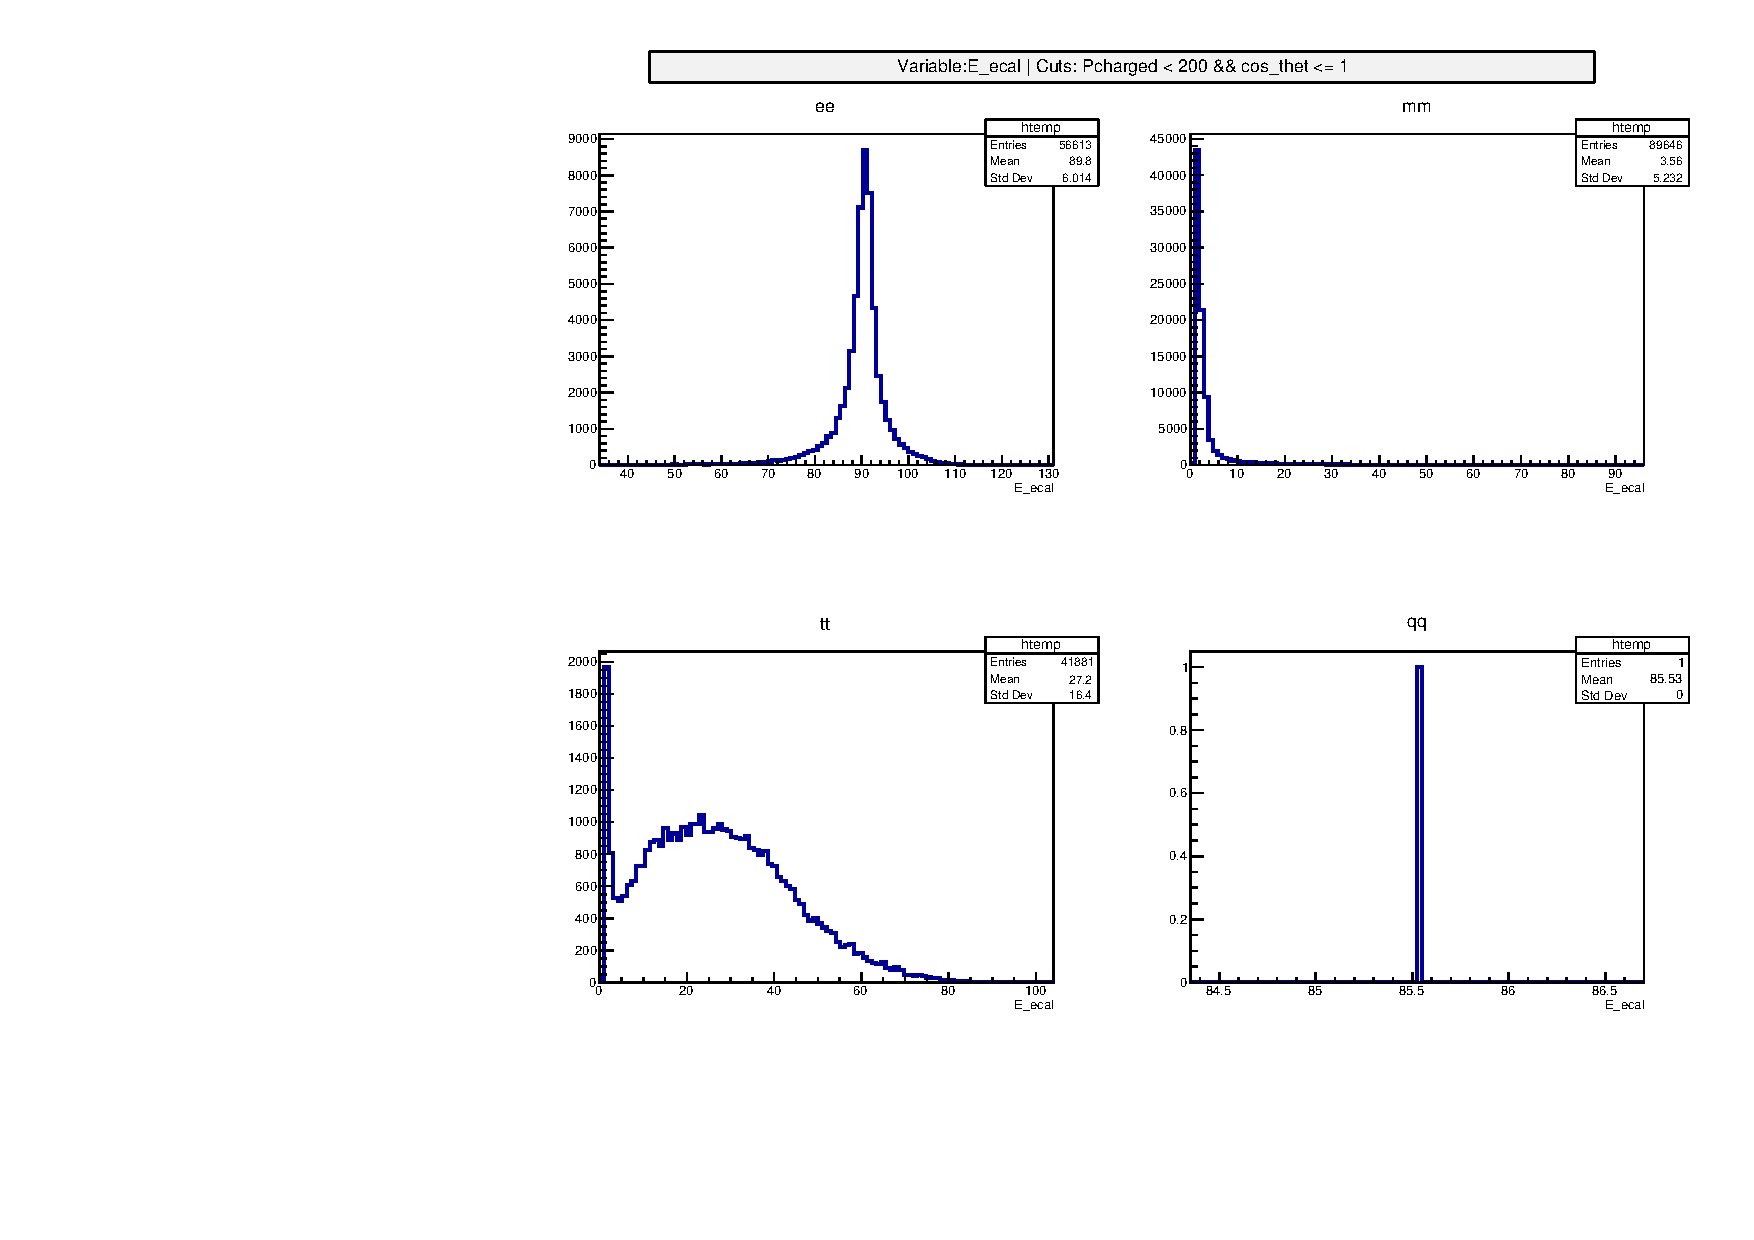
\includegraphics[width=0.8\linewidth]{ecal_before_ecal_cut.pdf}
	\cprotect\caption{\verb|E_ecal| distribution before \verb|E_ecal| cut for $ee$. }%
	\label{fig:ee_cuts}
\end{figure}
\begin{figure}[ht]
	\centering
	\includegraphics[width=0.8\linewidth]{hcal_after_Ncharged_ecal_cuts.pdf}
	\cprotect\caption{\verb|E_hcal| distribution after \verb|E_ecal| but before \verb|E_hcal| cut for $ee$.}%
	\label{fig:ee_cuts_hcal}
\end{figure}


For $\mu\mu$ selection, cut in \verb|Ncharged| is the same as $ee$: $\verb|Ncharged < 4|$. We have already seen in figure~\ref{fig:ee_cuts} that \verb|E_ecal| of $\mu\mu$ has a peak around $0$, so the \verb|E_ecal| cut for $ee$ gets inverted as cut for $\mu\mu$: $\verb|E_ecal| < 60$. Then remaining $\tau\tau$ events can be excluded with the help of \verb|Pcharged|, see figure~\ref{fig:mm_cuts}. $ee$ and $qq$ events are basically cut away, only unwanted events are $\tau\tau$. \verb|Pcharged| distributions of $\mu\mu$ and $\tau\tau$ are separated quite nicely, although some $\mu\mu$ events have $\verb|Pcharged| \approx 0$. A cut at $\verb|Pcharged| > 70$ will remove most of $\tau\tau$ events while preserve most of $\mu\mu$ events. After combinations of these cuts, $144$ $ee$ events, $83228$ $\mu\mu$ events, $480$ $\tau\tau$ events and zero $qq$ event survive.
\begin{figure}[ht]
	\centering
	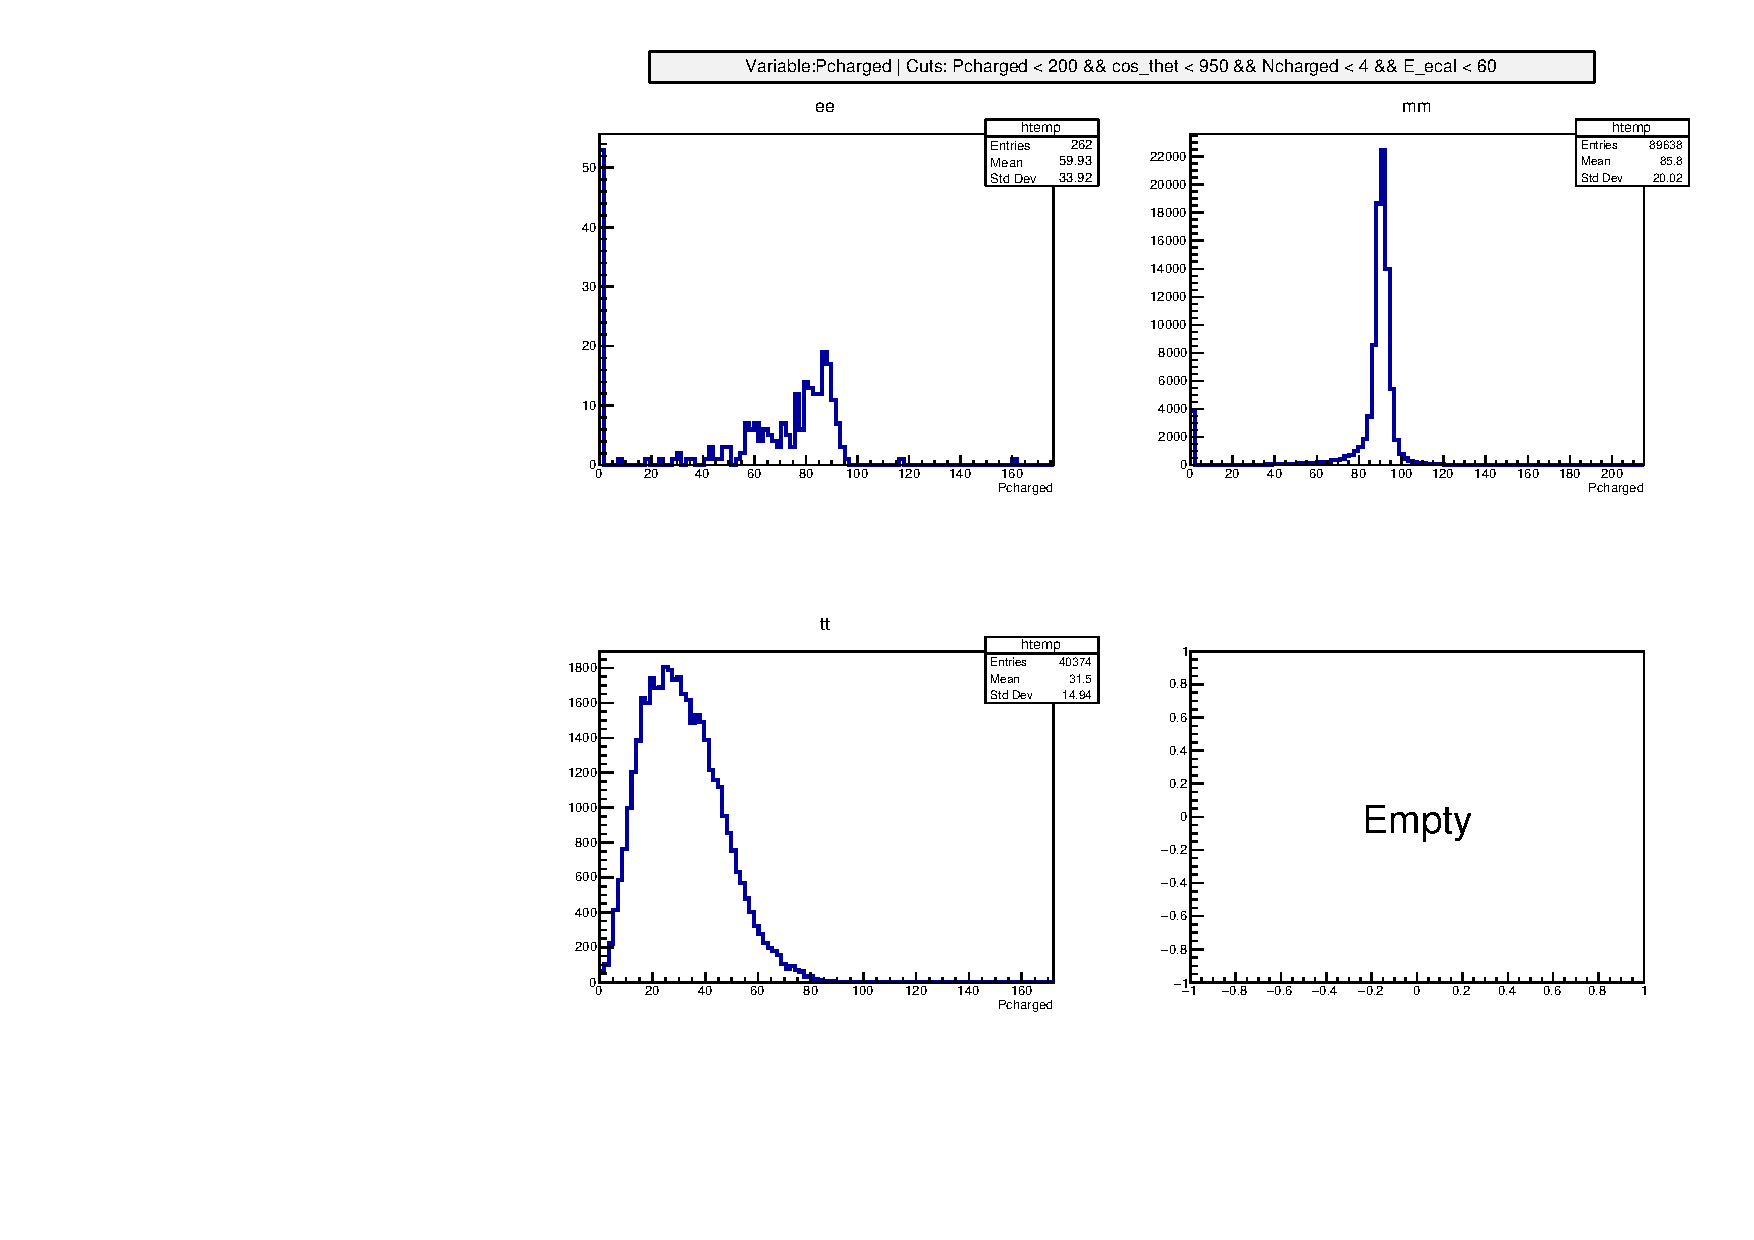
\includegraphics[width=0.8\linewidth]{Pcharged_mm_before_pcharged_cut.pdf}
	\cprotect\caption{\verb|Pcharged| distribution after \verb|E_ecal| cut for $\mu\mu$.}%
	\label{fig:mm_cuts}
\end{figure}

$\tau\tau$ can be picked out using the same cuts for $\mu\mu$ expect $\verb|Pcharged|$ cut gets inverted. Since there is a small peak at $\verb|Pcharged| = 0$ in $ee$ and $\mu\mu$ events, see figure~\ref{fig:mm_cuts}, a lower bound in \verb|Pcharged| should be set as well. Thus for $\mu\mu$: $1< \verb|Pcharged| < 60$. $E_ecal$ cut should be adjusted a bit. In figure~\ref{fig:ee_cuts}, there are still quite substantial amount of $\tau\tau$ event between $60 < \verb|E_ecal| < 70$. Thus we have for $\tau\tau$: $\verb|E_ecal| < 70$. Cut in \verb|Ncharged| is relaxed to $<5$ for better efficiency. After all these cuts, we have $243$ $ee$ events, $1446$ $\mu\mu$ events, $66990$ $\tau\tau$ events, and $38$ $qq$ events.

All the cuts are summarizes in table~\ref{tab:cuts_all}
\begin{table}[ht]
	\centering
	\begin{tabular}{cccccc}
		\toprule
	mode & \verb|cos_thet| & \verb|Pcharged| & \verb|Ncharged| & \verb|E_ecal| & \verb|E_hcal| \\
	\midrule
	$ee$ & $\leq 1$ & $< 200$ & $< 4$ & $>60$ & $< 2$ \\
	$\mu\mu$ & $\leq 1$ & $>70, <200$ & $<4$ & $<60$ & \\
	$\tau\tau$ & & $>1, <60$ & $<5$ & $<70$ \\
	$qq$ & & $<200$ & $>10$ & & \\
	\bottomrule
	\end{tabular}
	\caption{All cuts applied to select decay modes}
	\label{tab:cuts_all}
\end{table}

\paragraph{Channel selection}
